\chapter{{\scshape Steering Clear}: Reproduction Attempts}
\label{app:steering-clear}

\emph{The following chapter is a verbatim copy of a report that was sent to the original paper authors, \citet{steering-clear}, detailing the attempts to reproduce their work.}
\emph{The authors were quick to respond initially allowing the overall reproduction to be similar, however, they never responded to this report and the questions raised.}

\emph{The exact notation and wording is different from that used in the main thesis.}
\emph{This chapter simply contains the attempts made and associated data to demonstrate that reasonable effort was made to reproduce the exact results stated.}
\emph{Note that the dataset and model were rewritten from scratch as neither the dataset nor pre-trained model were found to be published online.}

I follow the original paper \cite{steering-clear} in all regards and any additional assumptions I make are explained below.
The paper describes the overview of how experiments were run but specific details are still missing allowing some room for interpretation.

I find that with a range assumptions across a number of trials that I am unable to fully reproduce the CAA plots the paper presents.
The primary issue I find is with the steerability metric stated in the paper, of total accuracy, where just the steered attribute accuracy results in a plot closer to the paper.

\section{Dataset}

This is a multi-label dataset:
\begin{itemize}[nolistsep]
    \item Each input is a 120 length vector representing 60 2-dimensional vectors. Each 2-dimensional vector is an ``attribute".
    \item Each label is a 60 length vector representing the target value of each of the 60 ``attributes". There are 8 target values.
    \item Each ``attribute" can take 8 values (the 8 target values) represented by a random vector from $\mathcal{N}(\mathbf{0}, \mathbf{I})$. Noise is added for each sample.
\end{itemize}

I only use $500,000$ examples rather than $2,000,000$ due to memory constraints but find that this does not affect model accuracy.
The paper does not state the exact method of generating anchor points but achieving ~100\% on the model should suffice.
I use a standard deviation of $0.01$ when adding noise to the samples thus insuring the datapoints are separable.

\section{Model}

A simple 4 layer MLP with:

\begin{itemize}[nolistsep]
    \item Layernorm after the 4 layers. This is fed into a classifier to predict the 60 labels.
    \item GeLU activation function.
    \item 512-512-256-512 hidden layer architecture.
    \item A 60 head classifier.
\end{itemize}

I test 3 types of residual streams:
\begin{itemize}[nolistsep]
    \item A single stream from input to layernorm.
    \item A residual over every single layer.
    \item No residual streams anywhere.
\end{itemize}

\begin{figure}
    \centering
    \begin{subfigure}{0.9\textwidth}
        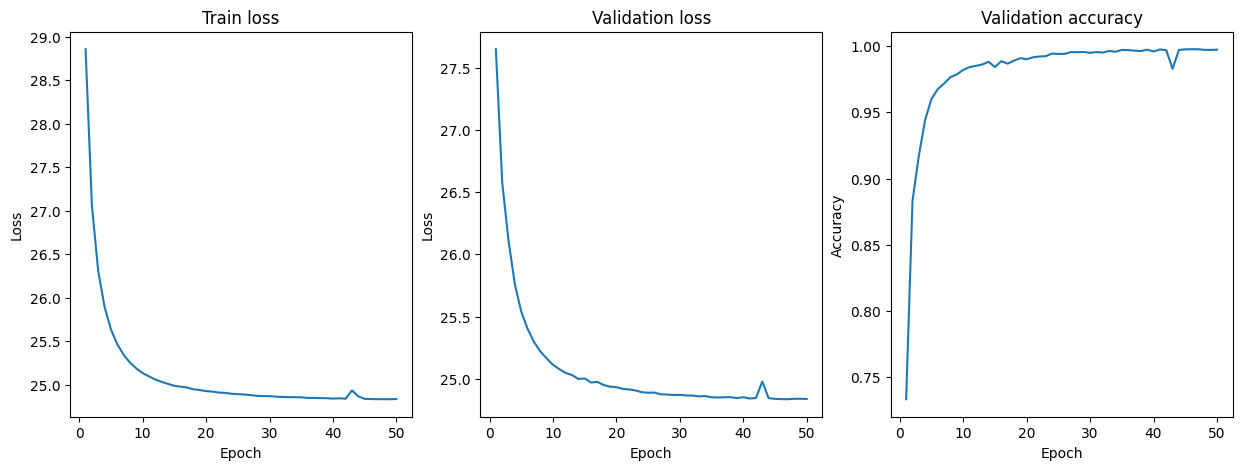
\includegraphics[width=\textwidth]{figures/no-residual-train-curves.png}
        \caption{Train and loss curves for the MLP without any residual streams.}
        \label{fig:nr-train-curves}
    \end{subfigure}

    \begin{subfigure}{0.9\textwidth}
        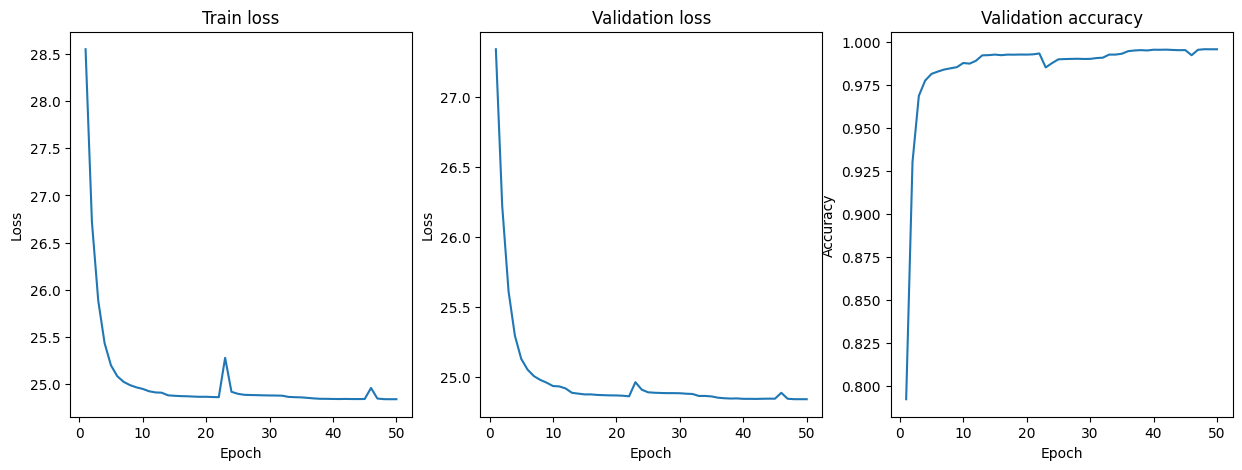
\includegraphics[width=\textwidth]{figures/residual-train-curves.png}
        \caption{Train and loss curves for the MLP with a residual stream per layer.}
        \label{fig:r-train-curves}
    \end{subfigure}

    \begin{subfigure}{0.9\textwidth}
        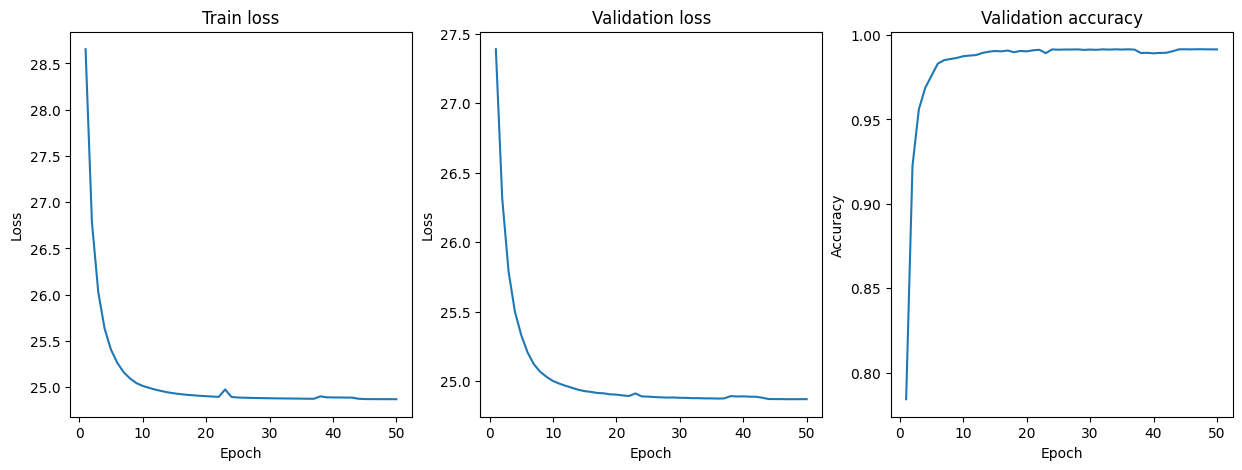
\includegraphics[width=\textwidth]{figures/single-residual-train-curves.png}
        \caption{Train and loss curves for the MLP with a single residual stream from input to layer-norm.}
        \label{fig:sr-train-curves}
    \end{subfigure}
\end{figure}

Figures \ref{fig:nr-train-curves}, \ref{fig:r-train-curves} and \ref{fig:sr-train-curves} show the train curves for the different models.
All of these eventually reach near 100\% accuracy.
The best model is chosen based on best validation accuracy and is chosen on the first instance of the best validation loss.

\begin{figure}
    \centering
    \begin{subfigure}{0.9\textwidth}
        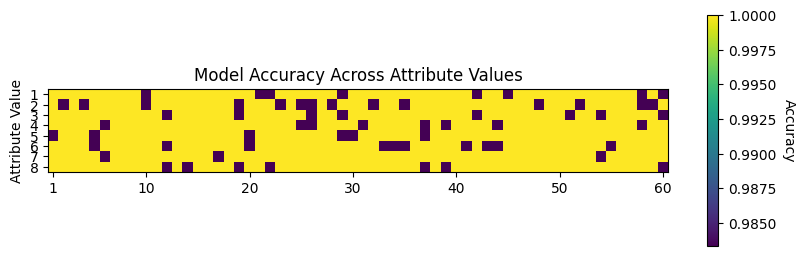
\includegraphics[width=\textwidth]{figures/no-residual-accuracy.png}
        \caption{The accuracy of the non-residual model on each attribute value.}
        \label{fig:nr-accuracy}
    \end{subfigure}
    \begin{subfigure}{0.9\textwidth}
        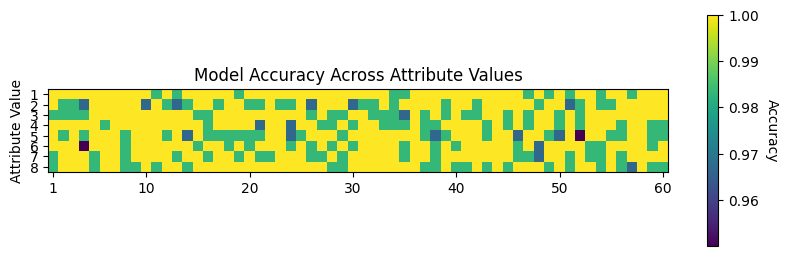
\includegraphics[width=\textwidth]{figures/residual-accuracy.png}
        \caption{The accuracy of the full residual model on each attribute value.}
        \label{fig:r-accuracy}
    \end{subfigure}
    \begin{subfigure}{0.9\textwidth}
        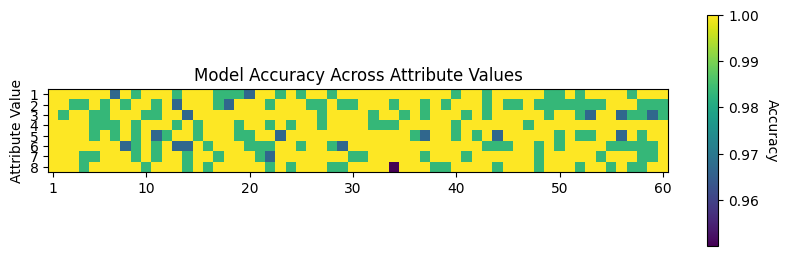
\includegraphics[width=\textwidth]{figures/single-residual-accuracy.png}
        \caption{The accuracy of the single residual model on each attribute value.}
        \label{fig:sr-accuracy}
    \end{subfigure}
\end{figure}

Figures \ref{fig:nr-accuracy}, \ref{fig:r-accuracy} and \ref{fig:sr-accuracy} show the accuracy of the model across all attributes and their values.
All other values are filled with a uniform random attribute.
All fills are presented to show that there is no bias towards a particular fill value.

From these plots I am fairly confident that my setup for the dataset and the training of the model is sound though there are clearly differences between how the residual streams are applied.

\section{Steering adaptor}

A forward hook is inserted at the 256-dim layer to extract activations for the contrastive pairs.
In the case of the residual stream per layer model the hook is inserted after the residual stream.

The inputs for generating the contrastive pairs are made as

\begin{itemize}[nolistsep]
    \item Selecting one attribute to target steering.
    \item Positive examples set this attribute to 0.
    \item Negative examples set this attribute to 1-7.
\end{itemize}

CAA simply takes the difference of means of these two activations as a steering vector.
A forward hook is registered at the same 256-dim layer which simply adds the scaled (parameterised by $\lambda$) steering vector to the output and returns it for the next layer.

To get repeated runs, a set of attributes is chosen\footnote{For ease of implementation these are just the first $n$ attributes} and the above process is applied to each.
In the end I run 20 repeats.

\begin{figure}
    \centering
    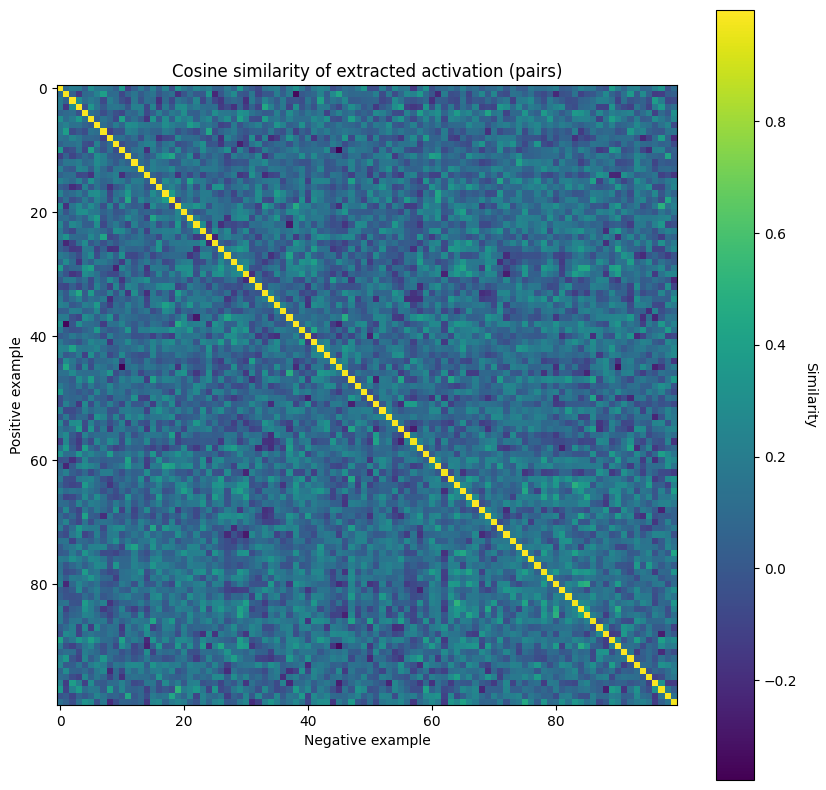
\includegraphics[width=0.9\textwidth]{figures/cosine-similarity.png}
    \caption{The cosine similarity between a sample of positive and negative pairs. This is for a specific attribute.}
    \label{fig:cosine-similarity}
\end{figure}

Figure \ref{fig:cosine-similarity} shows the cosine similarity of a sample of attributes.
The similarity between pairs is very high as expected as the other 59 attributes are identical.
The cross similarity is much lower showing that there is a variety of examples that are present when training the adaptor.
This plot is essentially the same across the models with minor differences in the exact similarity values.

\begin{figure}
    \centering
    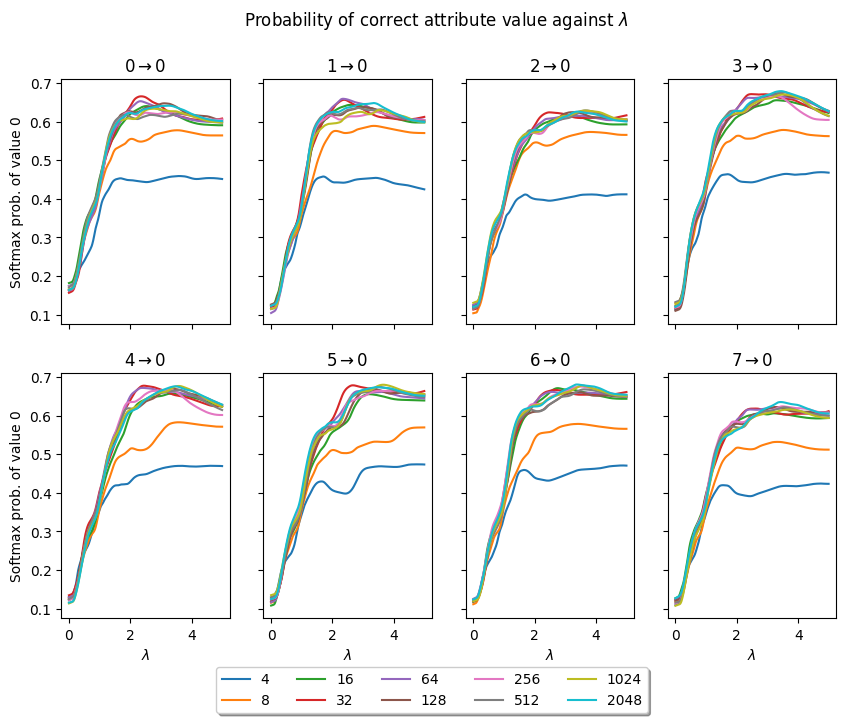
\includegraphics[height=0.4\textheight]{figures/no-residual-steering.png}
    \caption{The softmax probability of the target label (0) given the input label as a function of the scaling parameter $\lambda$. This is the model without any residual streams.}
    \label{fig:nr-steering}
\end{figure}

\begin{figure}
    \centering
    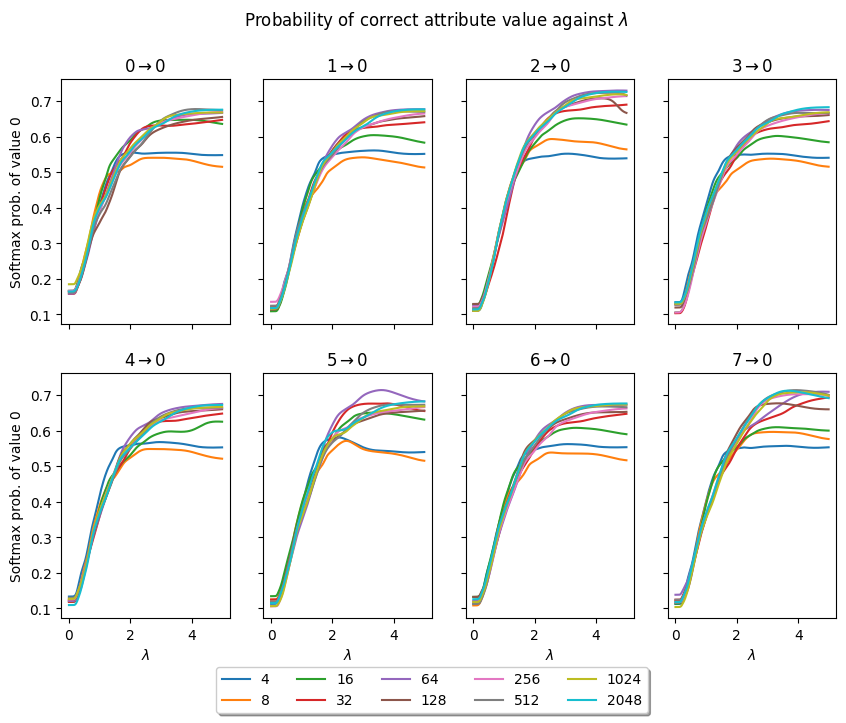
\includegraphics[height=0.4\textheight]{figures/residual-steering.png}
    \caption{The softmax probability of the target label (0) given the input label as a function of the scaling parameter $\lambda$. This is the model with a residual streams per layer.}
    \label{fig:r-steering}
\end{figure}

\begin{figure}
    \centering
    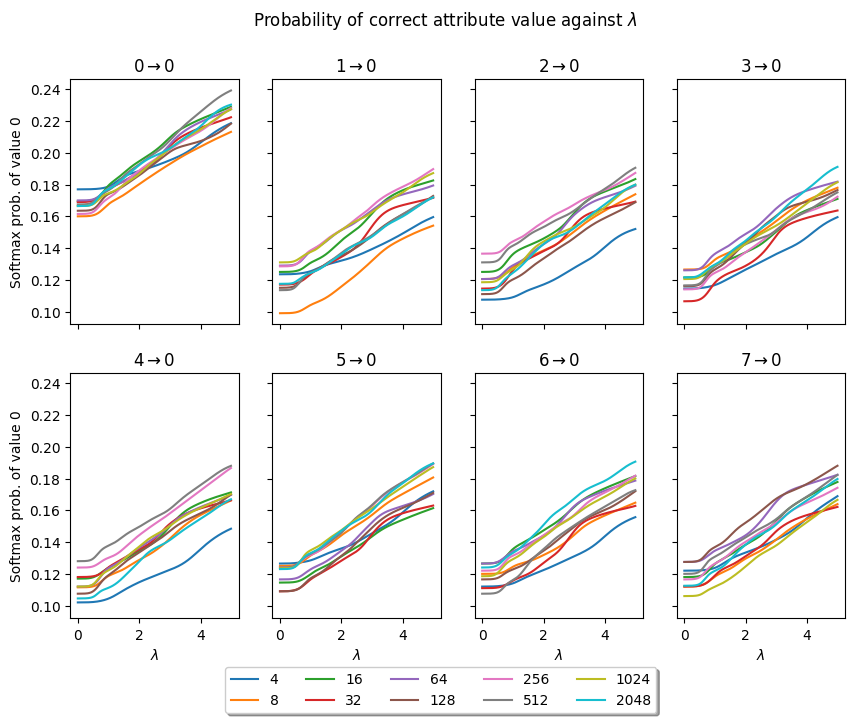
\includegraphics[height=0.4\textheight]{figures/single-residual-steering.png}
    \caption{The softmax probability of the target label (0) given the input label as a function of the scaling parameter $\lambda$. This is the model with a single residual stream from input to layernorm.}
    \label{fig:sr-steering}
\end{figure}

Figures \ref{fig:nr-steering}, \ref{fig:r-steering} demonstrate the effect of the CAA steering on the different attribute values for the target attribute.
The remaining attribute values are randomly selected.
The experiment is run over a range of example values for each 20 repeats and for each experiment the mean over 100 test inputs is returned.

Clearly demonstrated is that 4 and 8 examples do not achieve the same efficacy as the other examples regardless of the strength of the steering vector.
This does not take into account the effect on the attributes nor the softmax prob of the other values.
These experiments demonstrate that the steering vectors are able to steer effectively.

\section{Steering metric}

A subset of 1000 of the contrastive pairs above are withheld during training.
The negative generating inputs are fed through the model with the trained steering adaptor and the output recorded.
The goal is for the output to match the positive generating labels.

There are two metrics that I test:
\begin{itemize}[nolistsep]
    \item The accuracy on the steered attribute alone.
    \item The accuracy on all the attributes (this is the one stated in the paper).
\end{itemize}

\begin{figure}
    \centering
    \begin{subfigure}{0.45\textwidth}
        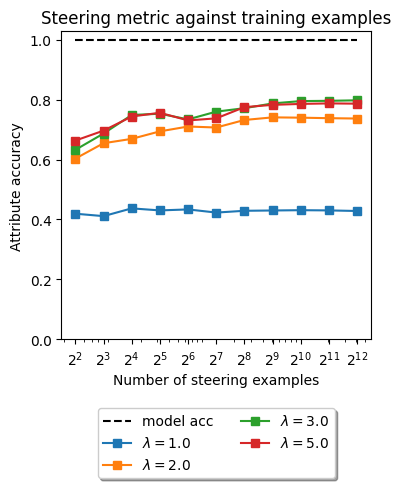
\includegraphics[width=\textwidth]{figures/no-residual-reproduction.png}
        \caption{Standard model steering accuracy on the steered attribute alone.}
        \label{fig:nr-reproduction}
    \end{subfigure}
    \hfill
    \begin{subfigure}{0.45\textwidth}
        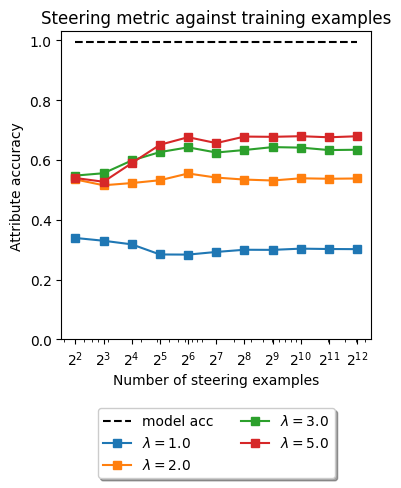
\includegraphics[width=\textwidth]{figures/residual-reproduction.png}
        \caption{Residual model steering accuracy on the steered attribute alone.}
        \label{fig:r-reproduction}
    \end{subfigure}
    \begin{subfigure}{0.45\textwidth}
        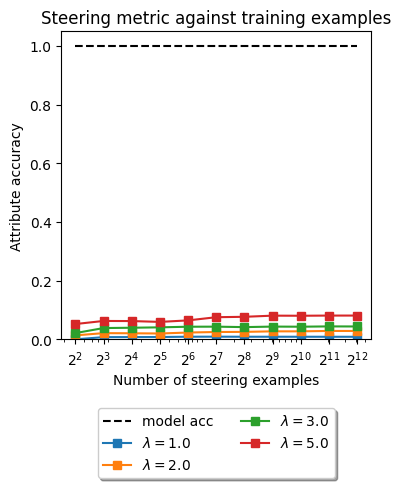
\includegraphics[width=\textwidth]{figures/single-residual-reproduction.png}
        \caption{Single residual stream model steering accuracy on the steered attribute alone.}
        \label{fig:sr-reproduction}
    \end{subfigure}
\end{figure}

Figures \ref{fig:nr-reproduction}, \ref{fig:r-reproduction} and \ref{fig:sr-reproduction} show the attempt at reproducing the paper figures for the top-left plot in Figure 1.
This only focuses on the CAA approach.
This uses a different metric to the paper focusing only on attribute accuracy rather than total accuracy and the trends are similar to those in the paper.
However, these plots are still not the same as the papers plots especially as they do not use the same metric.

\begin{figure}
    \centering
    \begin{subfigure}{0.45\textwidth}
        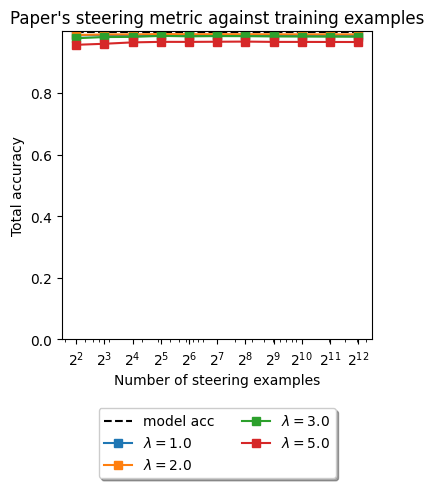
\includegraphics[width=\textwidth]{figures/no-residual-full-reproduction.png}
        \caption{Standard model steering accuracy on the steered attribute alone.}
        \label{fig:nr-correct}
    \end{subfigure}
    \hfill
    \begin{subfigure}{0.45\textwidth}
        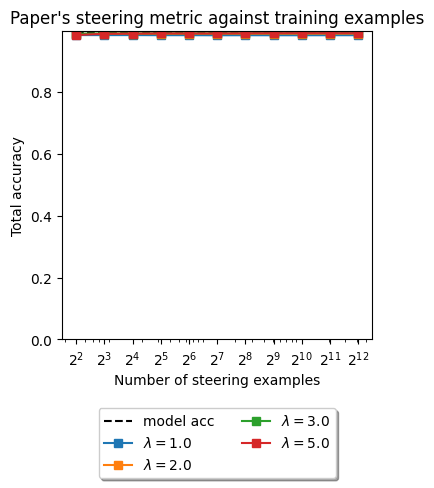
\includegraphics[width=\textwidth]{figures/residual-full-reproduction.png}
        \caption{Residual model steering accuracy on the steered attribute alone.}
        \label{fig:r-correct}
    \end{subfigure}
    \begin{subfigure}{0.45\textwidth}
        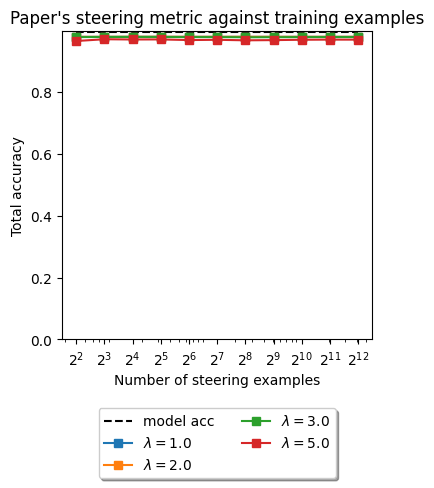
\includegraphics[width=\textwidth]{figures/single-residual-full-reproduction.png}
        \caption{Single residual stream model steering accuracy on the steered attribute alone.}
        \label{fig:sr-correct}
    \end{subfigure}
\end{figure}

Figures \ref{fig:nr-correct}, \ref{fig:r-correct} and \ref{fig:sr-correct} show the reproduction using the stated steering metric of total accuracy across all target labels.
